
%(BEGIN_QUESTION)
% Copyright 2007, Tony R. Kuphaldt, released under the Creative Commons Attribution License (v 1.0)
% This means you may do almost anything with this work of mine, so long as you give me proper credit

Looking at a minimalist RS-232 serial data network (now more properly known as TIA-232 or EIA-232 rather than RS-232), we see provision for data communication in two directions:

$$\includegraphics[width=15.5cm]{i02190x01.eps}$$

Answer the following questions about this simple serial network:

\begin{itemize}
\item{} Is this system capable of {\it simplex}, {\it half-duplex}, or {\it full-duplex} operation?  
\item{} Explain why the shield wire is connected to the Ground terminal only at one end, and not at both ends.
\item{} Explain what the term ``null modem'' means with reference to the cable connecting these two devices together, and why it is important we use this special cable for the job
\end{itemize}

\vskip 20pt \vbox{\hrule \hbox{\strut \vrule{} {\bf Suggestions for Socratic discussion} \vrule} \hrule}

\begin{itemize}
\item{} Identify a situation where we could get two serial devices to communicate with each other while using a ``straight-through'' cable rather than a ``null modem'' cable.
\item{} Suppose we needed to verify the communication of data in this system, and the only piece of test equipment we had was a digital multimeter (DMM).  Explain how we could use a DMM to sense digital data in this network.
\item{} A special tool useful for testing EIA/TIA-232 serial data lines is called a {\it breakout box}.  Research what a ``brekaout box'' is and how it may be used.
\end{itemize}

\underbar{file i02190}
%(END_QUESTION)





%(BEGIN_ANSWER)


%(END_ANSWER)





%(BEGIN_NOTES)

Actually, this system is theoretically capable of simplex, half-duplex, {\it and} full-duplex, but it is most commonly (and practically) used for half-duplex.  Just because two devices {\it can} talk to each other does not mean they must!  For this reason, the above system is capable of simplex (one-way) communication.  Half-duplex is not only possible, but with software handshaking it is the only practical form of duplex communication for EIA/TIA-232 data transfer.  Full duplex would be possible only without handshaking of any kind.

\vskip 10pt

Connecting the shield at one end only prevents the formation of a {\it ground loop} between the cable shield and the separate ground wire.

\vskip 10pt

A ``null modem'' cable is one where the transmit and receive wires cross, allowing two DTE devices such as this to directly communicate with each other.

%INDEX% Networking, serial: EIA/TIA-232 (formerly RS-232)

%(END_NOTES)


